\chapter{Application de quelques technologies Big Data sur l'analyse des  traceroutes} \label{chap:application-on-traceroutes}


\section{Introduction}

Ce chapitre reprend un ensemble de   technologies destinées  à la manipulation des données massives. Ce sont les technologies que nous avons expérimenté pour analyser des traceroutes disponibles dans le dépôt de RIPE Atlas. Précisément, ce sont les traceroutes permettant de tracer l'évolution du délai d'un lien comme c'est détaillé dans le chapitre \ref{chap:big-data-intro}.
% Nous allons présenter l'objectif de chaque technologie, ses avantages, ses inconvénients et ses limitations dans le cas de la présente analyse.
%Le présent chapitre reprend l'application de quelques technologies du Big Data manipulées en vue d'analyser le délai des liens. 
%On ne peut pas comparer ces technologies entre elles car elles ne se trouvent pas dans la même catégorie; quelques technologies n'assurent que le stockage, une autre technologie gère l'analyse ainsi que le stockage.  En revanche,
Les technologies que nous présentons  couvrent les besoins d'une ou de plusieurs étapes d'un processus d'analyse de données.
% (voir un exemple d'un processus d'analyse de données dans la section \ref{sec:process-data-analysis}). 
 
 %L'évaluation des performances  des technologies choisies est faite sur une machine ayant les caractéristiques reprises dans le tableau[!].

\section{Critères d'évaluation des technologies  Big Data}
Les critères d'évaluation d'une technologie Big Data  varient  suivant son objectif : stockage, calcul, etc.  En générale, la liste des critères que l'on peut considérer dans la comparaison des technologies Big Data est très longue.  Les critères sur lesquels nous  évaluons  les différentes technologies  Big Data expérimentées sont les suivants:
\begin{itemize}
	\item facilité de la mise en route et de la configuration de l'environnement de la technologie;
	\item flexibilité liée à la définition du  schéma de  données présentes dans les fichiers;
	\item temps d'exécution nécessaire pour fournir les résultats finaux d'une analyse de traceroutes;
	\item évolutivité de l'environnement Big Data mis en place pour des nouvelles données et de nouveaux besoins.
\end{itemize}

Dans la présente évaluation de quelques technologies Big Data, nous n'avons pas pris en compte d'autres critères. Car nous ne pouvons pas les évaluer. Par exemple, l'utilisation du  Big Data engendre des coûts  liés aux ressources nécessaires au stockage de données massives ainsi qu'au traitement de ces dernières. Nous avons donné des indications théoriques concernant les frais d'utilisation de deux technologies dédiées au stockage de données massives : Amazon S3 (voir le Tableau \ref{tab:pricing-s3-standard}) et MongoDB Atlas dont les frais d'utilisation  dépendent de plusieurs paramètres\footnote{Une estimation est possible suivant le fournisseur de cloud, elle est disponible  sur \url{https://www.mongodb.com/cloud/atlas/pricing}, consulté le $25/12/2018$.}. 

\section{Caractéristiques de l'environnement de test} \label{machine-openvz-caracteritics}

\paragraph{La machine de test} L'évaluation des technologies Big Data choisies sur un échantillon de traceroutes a été réalisé sur un conteneur de type OpenVZ ayant les caractéristiques suivantes :  système Debian GNU/Linux 7.11 (wheezy),  32,768 MB de  RAM, CPU MHz $ 2294.331 $.
%, nombre de CPUs $64$.

%Le Tableau \ref{tab:test-machine} présente les caractéristique de la machine sur laquelle nous avons effectué les différents tests. 
%\begin{table}[H]
%	\begin{tabular}{cc}
%		Type& OpenVZ container\\
%		RAM (MB)& 32768 \\
%		CPU & 64 (The logical CPU number of a CPU as used by the Linux kernel) \\
%	\end{tabular}
%	\caption{Caractéristiques de la machine de test}
%	\label{tab:test-machine}
%\end{table}
\begin{tcolorbox}
	Il existe différentes catégories de virtualisation. \textbf{OpenVZ} s'inscrit dans la catégorie Isolateur. Un isolateur est un logiciel permettant d'isoler l'exécution des applications dans des contextes ou zones d'exécution. Un conteneur OpenVZ  adopte un partitionnement logique au niveau des ressources systèmes : processus, réseau et système de fichier\footnote{Source : \url{http://cesar.resinfo.org/IMG/pdf/jtsiars-openvz_1_.pdf}, consultée le $29/12/2018$.}.
\end{tcolorbox}

Les différents tests effectués, présentés dans le présent chapitre, ont été effectués  au sein de cette machine. Nous notons qu'un seul test est lancé à un moment donné dans la machine.
\paragraph{Paramètres de l'analyse} Pour les paramètres de détection, nous avons utilisé les valeurs suivantes : \textit{timeWindow} est de $ 3600 $ secondes, l'intervalle de confiance est de $0,05$, \textit{alpha} est de $ 0,01 $ et \textit{minSeen} est de $3$. Les dates de début et de fin  varient suivant les traceroutes analysés.


\section{Collecte des traceroutes depuis le dépôt d'Atlas }
Nous avons utilisé l'API d'Atlas  comme source pour récupérer les traceroutes depuis le dépôt d'Atlas. L'API permet de collecter des traceroutes depuis le dépôt d'Atlas en ajustant quelques paramètres comme  l'identifiant de la mesure, la période souhaitée, etc. Toutefois, les données collectés doivent être réorganisées. Précisément, il faut passer d'un fichier d'une seule ligne qui contient une liste de traceroute à un fichier contenant plusieurs lignes et chaque ligne représente un traceroute. Nous avons manipulé des échantillons de traceroutes dont la taille entre $ 1 $ et $ 10 $ GO, ce sont des volumes  adaptés pour que la machine de test prenne en charge la récupération de ces volumes  et ensuite  réorganisation de ces traceroutes. 
La réorganisation des traceroute n'est pas nécessaire  MongoDB; l'import des traceroutes vers une base de données MongoDB peut être fait soit  via la liste des traceroutes ou bien via des lignes dans un fichier. Pour Amazon Athena et Spark, chaque traceroute doit occuper une  ligne dans les fichiers dans lesquels ils sont stockés. 

\section{Application 1 : MongoDB} \label{mongodb-impleme}
%\paragraph{ Application sur  MongoDB}~

%Les données relatives aux mesures traceroutes peuvent être récupérées de différentes manières. Par exemple,  les traceroutes à destination des instances du serveur DNS K-root. En ce qui concerne le travail de référence, les traceroutes sont récupérés à la fois par type d'adressage : IPv4 et IPv6 en se basant sur  l'identifiant  de la mesure : $ 5001 $, $ 6006 $, etc et par date.  Ainsi les

\paragraph{Evaluation des critères de sélection}~

MongoDB est la technologie Big Data utilisée par  Fontugne et al.  dans l'implémentation de l'outil de détection \cite{InternetHealthReport}. Dans MongoDB, les traceroutes sont organisés  dans des collections.  Chaque collection stocke les traceroutes effectués lors de la journée $YYYY\_MM\_DD$ et en adressage $V$. Par convention,  $V$  vaut $6$ s'il s'agit de l'adressage IPv6 et est vide.  La nomenclature  des collections permet de ne récupérer que les traceroutes concernés par l'analyse lancée. Le nom d'une collection est structuré comme suit: 	$tracerouteV\_YYYY\_MM\_DD$.
 

 
MongoDB est une technologie conçue pour assurer  le stockage de données dans un processus d'analyse de données. Nous avons utilisé la version locale de MongoDB, la quantité de données que nous pouvons stocker ainsi que le traitement appliqué sur les données récupérées dépendent principalement des ressources de la machine dans laquelle MongoDB est installé.
 
MongoDB est flexible en terme de définition du schéma de données; aucun schéma n'est requis.   Par exemple, dans certains cas, les traceroutes planifiés ne réussissent pas à atteindre une destination, dans ce cas, la structure de ces  traceroutes est différente  de la structure des traceroutes réussis. Les deux types de traceroutes sont stockés sans contrainte.

Les données stockées dans une collection MongoDB peuvent être manipulées en mode lecture et en mode écriture. Dans le premier, on cherche à lire des données en provenance de différentes sources. C'est le plus répandu dans les projets Big Data. Pour le deuxième mode, on peut mettre à jour un enregistrement dans une collection MongoDB. Ceci est moins fréquent dans les projets Big Data.

%Généralement l'analyse de données à grande échelle se limite qu'au mode lecture de données pour en tirer les connaissances. 
%MongoDB est adapté  aux projets visant la lecture de données massives mais aussi aux projets où on envisage la mise à jour d'un objet dans une collection (modification ou suppression). 
 
 MongoDB est évolutif; en cas de   mise à jour de la structure de nouveaux  objets traceroutes par Atlas,  cela n'affecte pas les données précédemment  stockées  dans MongoDB.
 
 %Malgré la convenance de MongoDB aux données non structurées et massives, l'utilisation de telle base de données, en version locale, nécessite l'ajustement de la machine locale où MongoDB tourne. 



%\paragraph{Les limitations de MongoDB}

%L'implémentation proposée de l'outil de détection utilise la version locale de la base de données MongoDB pour le stockage des données.  La quantité de données dont MongoDB peut stocker dépend de l'espace mémoire de stockage disponible dans la machine dans laquelle MongoDB est installé. De plus, les performances d'une détection lancée concernant une période donnée dépendent de la RAM de la machine en question. Pour conclure, l'utilisation de la version locale d MongoDB pour analyser les traceroutes à travers l'outil de détection dépend typiquement de la machine locale.
%\paragraph{Les performances de MongoDB}
\paragraph{Performances de la base de données MongoDB dans l'analyse des délais }~


Nous mesurons le temps écoulé durant l'analyse des traceroutes, stockés dans une base de données MongoDB,  en vue de détecter les anomalies dans le délai des liens. C'est le temps nécessaire à l'accomplissement des étapes de la phase I, de la phase II et de l'écriture des résultats dans un fichier. Chaque ligne de ce dernier  décrit un lien comme l'exemple donné dans le Listing \ref{resultLink}.  

Dans le Tableau \ref{tab:mongotiming-timing}, nous varions l'ensemble de traceroutes. Pour Chaque période, nous mesurons le temps nécessaire pour analyser les traceroutes capturés durant cette période pour plusieurs reprises. L'analyse de chaque période est fait $5$ fois, ce qu'on appelle ici des essais : Essai 1, Essai 2, etc.  Les traceroutes analysés sont ceux à destination des instances du f.root-servers.net\footnote{Voir les détails de la mesure 5004 sur \url{https://atlas.ripe.net/measurements/5004/}, consultée le $12/12/2018$}.

%en terme de stockage pour mesurer le temps nécessaire pour avoir  l'évolution de tous les liens présents dans  les traceroutes analysés, nous ne présentons que les premier trois essais. 


\begin{table}[h]
	\captionsetup{justification=centering}
	\resizebox{1\textwidth}{!}{
	\begin{tabular}{cccccccc}
\textbf{Période}&\textbf{Taille (bytes)}&\textbf{Essai 1 (s)}&\textbf{Essai 2 (s)} &\textbf{Essai 3 (s)}&\textbf{Essai 4 (s)}&\textbf{Essai 5 (s)}&\textbf{Médiane (s)} \\ \hline
$ 07/02/18 - 07/02/18 $&$  1,028,343,572 $&$  $&$  $&$  $ &&&\\ \hline 
$ 07/02/2018 - 08/02/2018 $&$  $&$  $&$  $&$  $ &&&\\ \hline 
$ 07/02/2018 - 09/02/2018 $&$  $&$  $&$  $&$  $ &&&\\ \hline 
$ 07/02/2018 - 10/02/2018 $&$  $&$  $&$  $&$  $&&&\\ \hline 
$ 07/02/2018 - 11/02/2018 $&$  $&$  $&$  $&$  $&&&  \\ \hline 
	\end{tabular}
}
\caption{Les temps d'exécution d'analyse de traceroutes en fonction de la taille de données avec MongoDB}
\label{tab:mongotiming-timing}
\end{table}

Nous reprenons les informations du Tableau \ref{tab:mongotiming-timing} dans la Figure \ref{fig:mongodbtiming}. L'axe  des abscisses représente la taille des fichiers contenant les traceroutes  analysés, appelée  $q$. L'axe  des ordonnées  représente le temps nécessaire à l'analyse d'une quantité  de traceroutes. Nous agrégeons les temps des différents essais et nous calculons  leur valeur minimale, maximale et la médiane.
Pour précision, le temps calculé est la différence entre l'instant  qui précède le lancement de l'analyse et l'instant qui suit la fin de l'analyse.

\begin{figure}[h]
	\centering
	\captionsetup{justification=centering}
	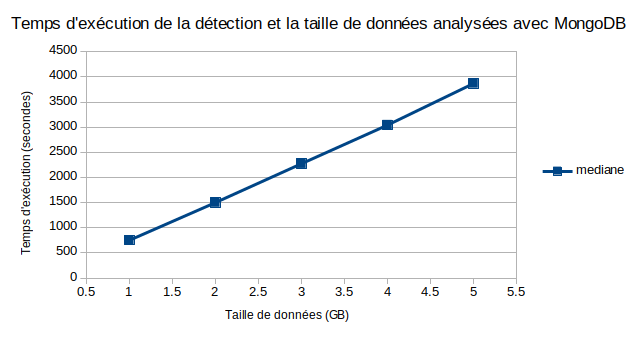
\includegraphics[width=0.7\linewidth]{illustrations/mongoDBtiming_0}
	\caption{}
	\label{fig:mongodbtiming}
\end{figure}

%Tandis que la  Figure \ref{fig:mongodbtiming}	 reprend la médiane  des temps d'exécution de la détection en fonction de  la taille de données analysées en utilisant MongoDB. 
%La Figure 	 \ref{fig:moustachemongodb} illustre la variation de la distribution des temps d'exécution. La Figure 	 \ref{fig:moustachemongodb} ainsi que la Figure \ref{fig:mongodbtiming} ont été obtenues en considérant les temps d'exécution de $10$ essais pour chaque taille de données.




%\begin{figure}[h]
%	\centering
%		\captionsetup{justification=centering}
%	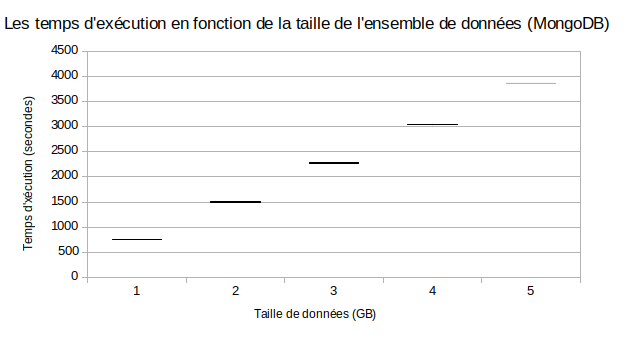
\includegraphics[width=0.7\linewidth]{illustrations/moustacheMongodb_0}
%	\caption{Les temps d'exécution en fonction de la taille de traceroutes analysés (MongoDB)}
%	\label{fig:moustachemongodb}
%\end{figure}

%La variation des temps d'exécution en fonction du nombre de traceroutes 


%Nous évaluons les temps d'exécution lors de l'analyse des délais des liens présents dans un ensemble de traceroutes, en utilisant MongoDB comme technologie de stockage de données massives.   

%On distingue deux types de variations : la taille de l'ensemble de données en terme de stockage et la taille en nombre de traceroutes présents dans l'ensemble de données.

%\begin{table}[h]
%	\captionsetup{justification=centering}
%	\resizebox{1\textwidth}{!}{
%		\begin{tabular}{cccccccc}
%			\textbf{Période}&\textbf{Taille (bytes)}&\textbf{Essai 1 (s)}&\textbf{Essai 2 (s)} %&\textbf{Essai 3 (s)}&\textbf{Essai 4 (s)}&\textbf{Essai 5 (s)}&\textbf{Médiane (s)} \\ %\hline
%			$ 07/02/18 - 07/02/18 $&$  1,028,343,572 $&$ 752,03 $&$ 750 $&$ 755,24 $ &&&\\ \hline 
%			$ 07/02/2018 - 08/02/2018 $&$ 2 $&$ 1499,28 $&$ 1504,98 $&$ 1503,62 $ &&&\\ \hline 
%			$ 07/02/2018 - 09/02/2018 $&$ 3 $&$ 2275,89 $&$2265,96 $&$ 2284,98 $ &&&\\ \hline 
%			$ 07/02/2018 - 10/02/2018 $&$ 4 $&$ 3035,19 $&$ 3043,21 $&$ 3057,45 $&&&\\ \hline 
%			$ 07/02/2018 - 11/02/2018 $&$ 5 $&$ 3871 $&$ 3889,57 $&$ 3894,5 $&&&  \\ \hline 
%		\end{tabular}
%	}
\section{Application 2 : Amazon DynamoDB}


%\paragraph{Application sur les traceroutes}~


L'élasticité est une des caractéristiques attirantes des services web d'Amazon. En particulier, c'est le cas d'Amazon DynamoDB. Ainsi, une implémentation basée sur Amazon DynamoDB  n'a pas à se soucier de la capacité  de stockage de données si la quantité de données évolue rapidement. 

 Amazon DynamoDB  n'assure que le stockage de données dans un processus d'analyse de données. La récupération et le traitement  des données stockées nécessitent l'ajustement des ressources de la machine qui reçoivent ces données, pareillement à MongoDB. La différence se situe à l'évolutivité implicite du stockage de données, qui ne se limite que par la capacité de stockage physique d'AWS. Tandis qu'une installation locale de MongoDB est liée aux ressources de la machine hébergeant ce dernier.  Nous n'avons pas expérimenté Amazon DynamoDB pour analyser les traceroutes, étant donné que notre évaluation des temps d'exécution est effectuée sur une machine locale, nous aurons les mêmes remarques que dans le cas de MongoDB en ce qui concerne l'ajustement des ressources de la machine qui reçoive les données.  
 
 A titre indicatif, une heure de tous les traceroutes effectués par toutes les sondes Atlas, concernant tous les identifiants de mesure,  fait une taille moyenne de  $620$ MB en format compressé, ce que représente une quantité d'environ $9$ GB en format texte.
%Toutefois,  au moment de de la récupération et de la manipulation de ces données, il faut ajuster les ressources pour pouvoir récupérer et traiter une quantité importante de données.

\section{Application 3 : Amazon S3, Amazon Glue  et Amazon Athena }

%\paragraph{Application sur les traceroutes}~
\paragraph{Vue générale}~

Nous avons combiné les trois services d'Amazon (Amazon S3, Amazon Glue  et Amazon Athena)  afin de créer un environnement d'analyse de données massives. 
Un des scénarios possibles mettant en pratique ensemble ces trois services est illustré dans la Figure
\ref{fig:gluecrawler}\footnote{Amazon Redshift  est un entrepôt de données et  Amazon Quicksight  est un service cloud d'informatique décisionnelle.}. Nous détaillons chaque services dans les sections suivantes.

Afin d'utiliser Amazon Athena pour l'interrogations des traceroutes stockés dans des fichiers, nous avons besoin d'abord de stocker les fichiers dans Amazon S3. De plus, nous avons besoin de créer un  schéma de données. Il s'agit de créer une table comme les tables dans un SGBDR. Chaque enregistrement dans cette table correspond à une ligne dans les fichiers de données censés être lus par cette table. Il existe deux manières pour créer une table dans Athena : en utilisant Amazon Glue ou création manuelle. \textit{traceroutes\_api} désigne le nom de la table reprenant tous les traceroutes.
%Une vue globale du  processus de l'analyse  est illustré dans la Figure  

\begin{figure}[h]
	\centering
	\captionsetup{justification=centering}
	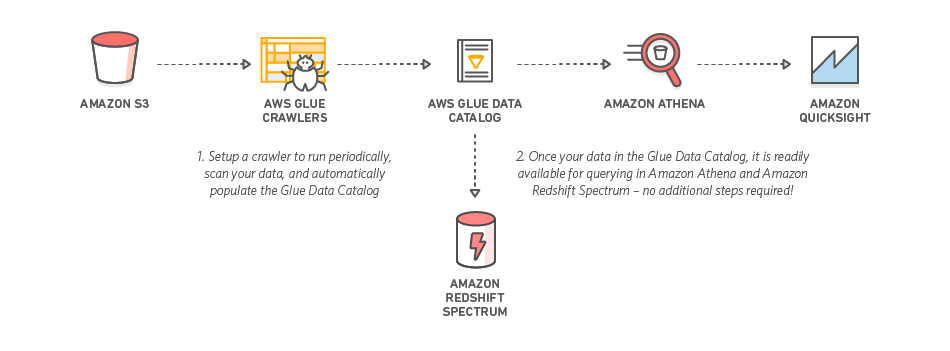
\includegraphics[width=1\linewidth]{illustrations/glue_crawler}
	\caption{Une combinaison des services web d'Amazon : Amazon S3, Amazon Glue, Amazon Athena, Amazon Quicksight  et Amazon Redshift}
	\label{fig:gluecrawler}
	\source{\url{https://docs.aws.amazon.com/fr_fr/athena/latest/ug/glue-best-practices.html}, consultée le $16/05/2018$.}
\end{figure}


\paragraph{Création de la table traceroutes avec Amazon Glue}~

Nous avons lancé    la détection automatique du schéma, avec Amazon Glue, d'un ensemble de  traceroutes enregistrés dans un fichier faisant une taille de $500$ MB. Toutefois, la détection a échoué. Autrement dit, Amazon Glue n'a pas pu inférer le schéma d'une seule table capable de lire tout traceroute dans ce fichier.  L'échec de l'inférence est dû au fait que le fichier contient des traceroutes différents en terme de structure, car la structure dépend de la version du firmware de la sonde ayant effectué le traceroute. Les différentes versions du firmware  pour chaque type de mesure sont détaillées dans le site Web d'Atlas\footnote{\url{https://atlas.ripe.net/docs/data_struct/}, consultée le $16/01/2018$.}.
 %L'origine de cette différence  est le fait que ces traceroutes ont été effectués par des sondes ayant un firmware différent. Car le contenu des résultats d'une requête traceroute  et son organisation dans un objet JSON dépend partiellement du firmware de la sonde. 
 
\paragraph{Création manuelle de la table \textit{traceroutes\_api}}~

Nous avons créé la structure de la table \textit{traceroutes\_api}  manuellement en se basant sur la structure détaillée d'une réponse traceroute pour chaque version du firmware. Les différentes structures de réponses d'une requête traceroute n'a posé aucun problème dans la création manuelle de la table. Dans notre cas, la réussite de la création manuelle est due au fait que les attributs dont l'outil de détection a besoin sont présents dans toutes les versions du firmware d'une part. D'autre part, Amazon Athena est flexible en ce qui concerne l'association entre un objet JSON et un enregistrement dans une table. Autrement dit, si un attribut existe dans l'objet JSON, la colonne correspondante prend sa valeur et vide dans le cas échéant.  

\paragraph{Partitionnement des données stockés dans Amazon S3}~

Nous avons   pris en compte  le partitionnement de données dans un compartiment S3 dans la création de la table \textit{traceroutes\_api}.  L'utilisation du partitionnement est optionnel. 
Le partitionnement  de données présentes dans un compartiment Amazon S3 permet de limiter la quantité de données à analyser par une requête Amazon Athena. Le partitionnement améliore  les performances d'Amazon Athena. D'une part, la requête s'exécute rapidement. D'autre part, le partitionnement réduit les coûts engendrés  suite à l'utilisation d'Amazon Athena, car ce dernier est facturé selon la quantité de données analysées. En pratique,  une partition créée joue un rôle similaire à celui d'une colonne durant l'interrogation d'une table dans Athena. 

Prenons un exemple illustrant l'apport du partitionnement. Nous avons des traceroutes effectué en adressage IP la version  $ 4 $ et $ 6 $.


\textit{af\_} désigne le type d'adressage : \textit{af\_} vaut $4$ en cas d'adressage IPv4 et $6$ en cas d'adressage IPv6. Sans l'utilisation du partitionnement et si on ne souhaite récupérer que  les traceroutes ayant comme adressage IPv4, tous les traceroutes présents dans le compartiment S3 (appelé \textit{s3://ripeatlasdata}), dédié au stockage des traceroutes récupérés depuis le dépôt d'Atlas, sont évalués\footnote{L'évaluation du type  d'adressage est effectué selon la valeur de l'attribut \textit{af} d'un traceroute, il vaut \textit{4} ou \textit{6}.}.

Toutefois, en partitionnant les données suivant par exemple le type d'adressage, seuls les fichiers dans la partition\footnote{Partition dans le sens d'Amazon Athena.} af\_ = 4 qui sont analysés. Par conséquent, le partitionnement permet de réduire les coûts d'utilisation du service Amazon Athena, surtout si la quantité de données est très importante. 


Les partitions   créées sont illustrées  dans la Figure 	\ref{fig:partitionnement-athenaa}. Nous détaillons les différentes partitions dans le Tableau \ref{tab:partition-description}. Nous donnons le nom de la partition dans la première colonne, quelques valeurs de chaque partition dans la deuxième colonne et la troisième colonne de ce tableau reprend une description de la partition.

\begin{figure}[H]
	\centering
	\captionsetup{justification=centering}
	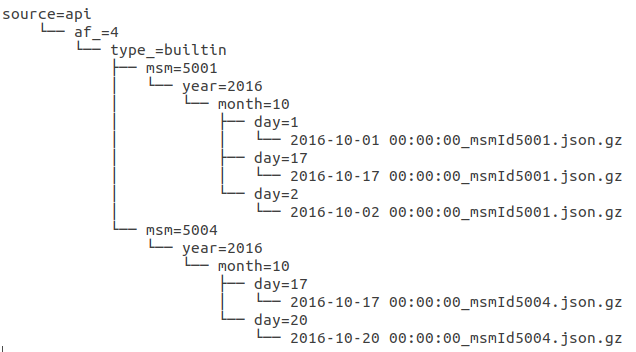
\includegraphics[width=1\linewidth]{illustrations/partitionnement-athena}
	\caption{L'organisation des traceroutes dans le compartiment Amazon S3 \textit{s3://ripeatlasdata}}
	\label{fig:partitionnement-athenaa}
\end{figure}

\begin{table}
		\centering
		\captionsetup{justification=centering}
\begin{tabular}{|c|c|l|}
	\hline 
\textbf{partition}	& \textbf{Valeurs} & \multicolumn{1}{c|}{\textbf{Commentaires} }\\ 
	\hline 
 source& api & Les  traceroutes récupérés depuis le dépôt  d'Atlas via l'API \\ 
	\cline{2-3}
	 &typeanddate& Les  traceroutes récupérés depuis la page Web\\
	\hline 
	af\_& 4  & Les traceroutes en adressage IPv4 \\ 
	\cline{2-3} &6& Les traceroutes en adressage IPv6\\	\hline 
	type& builtin  & Les traceroutes en provenances des mesures intégrées \\ 
	\cline{2-3} 
 &anchor& Les traceroutes à destinations des ancres\\ \hline
	msm& 5001 & Les traceroutes ayant msm\_id = 5001 \\ 
	\cline{2-3}  &5004& Les traceroutes ayant msm\_id = 5001 \\
	\hline 
	year& 2016 & Les traceroutes effectués en $2016$ \\ 
	\hline 
	month& 10 & Les traceroutes effectués en octobre \\ 
	\hline 
	day& 1 & Les traceroutes effectué le premier du mois \\ 
	\hline 
\end{tabular}
\caption{Exemple des partitions créées dans un compartiment Amazon S3} 
\label{tab:partition-description}
\end{table}

 Les   partitions \textit{af\_} et \textit{type\_} sont nommée de cette manière, au lieu de \textit{af} et \textit{type} car  la table \textit{traceroutes\_api} contient des colonnes avec ces noms et comme les partitions agissent comme des colonnes  lors de l'évaluation d'une requêtes avec Amazon Athena, les noms de ces partitions ont été adaptés.

Par exemple, les traceroutes qui se trouvent dans  le fichier

 \textit{2016-10-01 00:00:00\_msmId5001.json.gz} sont analysés par toute requête Athena  
impliquant les partitions d'une des manières suivantes : 
(source = api) ou (source = api et af\_ = 4) ou (source = api et af\_ = 4 et type = builtin) ou (source = api et af\_ = 4 et type = builtin et msm = 5001) ou 
(source = api et af\_ = 4 et type = builtin et msm = 5001 et year = 2016) ou (source = api et af\_ = 4 et type = builtin et msm = 5001 et year = 2016 et month = 10) ou
 (source = api et af\_ = 4 et type = builtin et msm = 5001 et year = 2016 et month = 10 et day = 1).

\paragraph{Interrogation des données Avec Amazon Athena}~

Une fois les fichiers de données  synchronisés vers le compartiment AWS S3 et le schéma  de données  créé, on passe à l'interrogation de données en utilisant les requêtes SQL basées sur Presto.  
Nous donnons un exemple d'une requête Athena dans la section \ref{sql-athena-request} de l'annexe \ref{athena-appendix}.

\paragraph{Intégration d'Amazon Athena dans l'outil de détection}~ \label{integration-aws-possibilite-une}
 

Pour intégrer Amazon Athena dans l'outil de détection \cite{InternetHealthReport}, on distingue deux possibilités. La première possibilité n'utilise Athena que pour récupérer  les traceroutes stockés dans Amazon S3 vers  la machine locale. Ensuite, cette dernière poursuit les traitements  décrits dans la phase I et II. Dans ce cas, nous ne profitons pas  des performances d'Amazon Athena vu que les traitements complexes sont effectués dans la machine locale.
%vérifiés en terme de validité; c'est l'objectif des étapes $1$ et $2$ dans le processus de la création de l'évolution des RTTs différentiels des liens (voir la section \ref{steps-rtt-analysis}).  
 %Les traitements qui suivent (étapes  à partir de $3$) sont effectués dans la machine locale. Dans ce cas, l'utilisation des technologies  Big Data est limité qu'au niveau stockage de données massives. 

Tandis que  la deuxième possibilité vise la maximisation des traitements des deux phases I et II au sein de l'infrastructure  d'Athena. De ce fait, la machine locale n'a qu'à recevoir les derniers résultats de la détection, voire les résultats finaux. Pour cette deuxième possibilité, les données doivent être manipulées de sorte à maximiser,  	au niveau d'Amazon Athena,  les traitements relatifs à toutes les étapes des deux phases I et II. 

Pour la deuxième possibilité, le défi est de trouver la requête ou bien l'ensemble de requêtes SQL à exécuter sur Athena en vue d'avoir l'évolution du RTT différentiel des liens. 
Vu la complexité des  étapes des phases I et II, on ne peut pas trouver une seule requête SQL assurant toutes ces étapes à la fois. Supposons qu'il existe une requête SQL capable de trouver les liens possibles avec leurs RTTs différentiels : à l'étape $ 4 $ dans \ref{steps-rtt-analysis}, on construit la distribution des RTTs différentiels pour tout lien $l$ identifié dans les traceroutes de la période $d_k$. Cette distribution est mise à jour à chaque fois $l$ est identifié dans un des traceroutes  de la période $d_k$. 

Soient  $T_k$ = \{$t_{k, j}$\}  l'ensemble de traceroutes effectués durant $d_k$, avec $j \in [1, R_k]$ et $R_k$ est le nombre de traceroutes effectués durant $d_k$. Nous décrivons le parcours des traceroutes d'une période $d_k$ brièvement dans le pseudo-code \ref{alo-inference-link}. Nous n'avons pas donné  tous les détails, car l'objectif est d'évaluer la convenance d'Athena au traitement souhaité.
\begin{algorithm}[H]
\begin{algorithmic}[1]
	 \ForAll{ $t_{k, j}$ $\in$ $T_k$} \
	  \State $links$ $\leftarrow$ getLinksFromTraceroute($t_{k, j}$)
	  	 \ForAll{$l$ $\in$ $links$}
	  	 		\State updateLinkRttDistribution($l$) \label{update-link}
	  	 \EndFor
	 \EndFor
\end{algorithmic}
\caption{Une partie de l'étape $4$ du processus de la détection des anomalies des délais }
\label{alo-inference-link}
\end{algorithm}

Avec : 
\begin{itemize}
	\item \textit{getLinksFromTraceroute($t_{k, j}$)} énumère tous les liens possibles dans le traceroute $t_{k, j}$.

    \item \textit{updateLinkRttDistribution($l$)} ajoute le RTT différentiel calculé du lien $l$ à la distribution des RTTs différentiels courante de ce lien pour la période $d_k$.
\end{itemize}


Le service Athena est conçu pour la lecture de données, toute mise à jour de données n'est pas possible avec ce service. C'est pourquoi la distribution des RTTs différentiels de chaque  lien identifié doit être sauvegardée dans un endroit accessible en lecture et en écriture, par exemple dans un compartiment AWS S3. Que ce soit un fichier reprenant la distribution des RTTs différentiels  par un seul lien ou bien un fichier pour tous les liens,   à la ligne  \ref{update-link} du pseudo-code \ref{alo-inference-link}, un fichier doit être lu et mise à jour avec de nouvelle valeur. Pour une période $d_k$ d'une heure, le nombre de traceroutes est de l'ordre de milliers. Chaque traceroute $t_{k,j}$ peut inclure $L_{k,j}$ liens. Dans ce cas, le nombre total, d'une période $d_k$, de mise à jour de la distribution des RTTs différentiels est    $ \sum_{m=1}^{R_k}  L_{k,m}$. $ L_{k,j} $ dépend du nombre de saut du  traceroute $t_{k,j}$.

 %de l'ordre $R_k$\texttimes$L$ de fois.  Cette estimation est à titre indicatif, de plus elle ne concerne que l'étape $4$, le nombre de lectures et/ou d'écritures dépend des requêtes SQL créées pour les autres étapes. 

En plus du nombre de lectures et d'écritures, relatives à la phase I, que nous venons de décrire, à la phase II, la détection des anomalies s'effectue en  comparant les intervalles de confiances : un intervalle de confiance courant du lien avec celui de référence. Cette comparaison révèle deux contraintes. La première contrainte concerne  la fonction permettant de calculer les deux bornes de l'intervalle de confiance de Wilson ne fait pas partie des fonctions disponibles sur Amazon Athena. D'autre part, Amazon Athena ne permet pas la création des fonctions personnalisées pour répondre à des besoins non couverts par Amazon Athena. La deuxième contrainte concerne la mise à jour de l'intervalle de confiance de référence qui doit être faite à chaque nouvelle période.


\paragraph{Evaluation des critères pour Amazon S3 et Amazon Athena  }~

Afin d'utiliser le service Amazon Athena à moindre coût, il est conseillé d'utiliser le partitionnement, car moins de frais sont appliqués. Si un partitionnement particulier est adopté, la création du schéma de données est basé sur ce partitionnement ainsi que les requêtes SQL destinés à l'interrogation de la table de données.

En ce qui concerne l'évolutivité d'une application basée sur ces deux services d'Amazon, on note que toute mise à jour de la structure de données des objets traceroutes peut affecter l'entièreté de la configuration initiale. A savoir, l'organisation des fichiers de données via le partitionnement, le schéma de données et les requêtes SQL.

 Quant à la flexibilité du schéma de données, le service  Amazon Athena est tolérant au données manquantes. Etant donné que la structure d'un objet traceroute dépend de la version du firmware de la sonde, nous avons créé trois schémas de tables. La première table  modélise tout objet traceroute de  version $5$, la deuxième modélise tout objet traceroute de version $6$ et enfin la troisième table modélise ceux ayant la version $7$. En expérimentant différentes requêtes, nous avons conclu  que Amazon Athena a pu récupérer les données de la version récente ($7$) via le schéma de la version $5$ malgré que la version $7$ a plus d'attributs par rapport à la version $5$.
 
%Avec une autre technologie qui travaille en mémoire, les résultats sont données plus rapidement. 

\paragraph{Performances des services Amazon S3 et Athena dans l'analyse des délais }~ \label{aws-perforsm}

Nous avons utilisé Amazon Athena et Amazon S3 pour analyser les traceroutes et détecter les anomalies des délais. Nous précisons que nous avons évalué la première possibilité décrite dans la section \ref{integration-aws-possibilite-une}. Nous avons bénéficié de la  possibilité  de lancer des requêtes destinées à Amazon Athena à travers l'API REST, précisément en Python. Et comme l'implémentation proposée par les auteurs du travail de référence est écrite en Python, nous avons adapté cette implémentation de sorte  de récupérer les traceroutes depuis   depuis Amazon S3 via Amazon Athena au   lieu de le faire depuis la base de données locale MongoDB.  

Etant donné que nous avons utilisé le partitionnement de données, une analyse des délais nécessite d'autres paramètres à ajuster en plus de ceux relatifs à la détection. Ce sont les paramètres permettant de sélectionner les traceroutes présents sur Amazon S3. Du fait que le partitionnement de données (voir une partie de l'arborescence dans la Figure 	\ref{fig:partitionnement-athena}) est réalisé sur base du type de traceroute (\textit{builtin} ou \textit{anchor}) et de l'identifiant de la mesure ($ 5004 $, $6001$, etc) qui a enregistré un traceroute, nous devons personnaliser  la requête visant la   récupération des traceroutes  depuis Amazon S3 pour qu'elle prennent en compte aussi les partitions.

Le Tableau \ref{tab:athena-data} contient les temps d'exécution suivant la taille de l'ensemble de données donné en entrée de la détection.

\begin{table}[H]
	\centering
	\captionsetup{justification=centering}
\begin{tabular}{c c c}
	\textbf{Période} & \textbf{Taille(GB)} & \textbf{Temps (secondes) } \\ 	\hline 
$ 07/02/18 - 07/02/18 $	&$ 1 $&	$ 1898.31 $ \\ 	\hline 
$ 07/02/2018 - 08/02/2018 $	&$ 2 $&	$ 3533.6562171 $ \\ 	\hline 
$ 07/02/2018 - 09/02/2018 $&	$ 3 $&	$ 5284.91494989  $ \\ 	\hline 
$ 07/02/2018 - 10/02/2018 $	&$ 4 $&$ 	7228.88 $  \\ 	\hline 
$ 07/02/2018 - 11/02/2018 $	&$ 5 $& $ 8984.873281	 $ \\ 	\hline 
\end{tabular} 
\caption{Les temps d'exécution par taille de l'ensemble de données (Amazon Athena et Amazon S3)}
\label{tab:athena-data}
\end{table}

Nous distinguons trois phases dans cette approche (approche 1). Premièrement,  les données sont récupérées depuis Amazon S3. Plusieurs facteurs affectent cette étapes, par exemple,  les conditions du réseau, les ressources allouées par Amazon pour répondre à chaque requête  Athena à destination des données disponibles sur Amazon S3, l'optimalité de la requête SQL, etc.  En deuxième lieu, les résultats de la requête doivent être désérialisés pour pouvoir les utiliser localement. Enfin, sur base des données récupérées, la détection des anomalies peut être déclenchée.
%
%
%Nous évaluons les temps d'exécution de plusieurs  analyses de délais lancées en variant la taille de données. Rappelons qu'il s'agit de la première possibilité: Amazon S3 pour le stockage de traceroutes et Amazon Athena pour récupérer les traceroutes valides, le reste de traitements sont effectués au sein de la machine locale.  Le Tableau	\ref{tab:awstiming-timing} reprend plus de détails. 
%\begin{table}[H]
%	%\begin{threeparttable}
%	
%	\captionsetup{justification=centering}
%	\begin{tabular}{ccccc}
%		\textbf{Début - fin} &\textbf{Durée (jours)}  & \textbf{Taille}  & \textbf{Nb traceroutes} & \textbf{Temps (secondes)} \\ \hline
%		
%		07/02/2018             &1 &1 GB&& 3870\\ \hline
%		07/02/2018 - 08/02/2018&2 &1 GB&& 2942\\ \hline
%		07/02/2018 - 09/02/2018&3 & 1 GB&& 2991\\ \hline
%		07/02/2018 - 10/02/2018&4 & 3 GB&& 20955\\ \hline
%		07/02/2018 - 11/02/2018&5& && \\ \hline
%		07/02/2018 - 12/02/2018&6& && \\ \hline
%		07/02/2018 - 13/02/2018&7& && \\ \hline
%		07/02/2018 - 14/02/2018&8& && \\ \hline
%		07/02/2018 - 15/02/2018&9& && \\ \hline
%		07/02/2018 - 16/02/2018&10& && \\ \hline
%		07/02/2018 - 17/02/2018&11& && \\ \hline
%		07/02/2018 - 18/02/2018&12& && \\ \hline
%		07/02/2018 - 19/02/2018&13& && \\ \hline
%		07/02/2018 - 20/02/2018&14& && \\ \hline
%	\end{tabular}
%	\caption{La moyenne des temps d'exécution d'analyse de traceroutes en fonction de la taille de données avec Amazon S3 et Amazon Athena }
%	\label{tab:awstiming-timing}
%\end{table}
La Figure \ref{fig:temps-avec-aws} présente un seul essai pour chacune des tailles utilisées auparavant avec MongoDB.  Le temps de chaque essai comprend l'étape de la récupération des traceroutes depuis Amazon S3, le temps de préparation des traceroute et enfin le temps de la détection des anomalies. Autrement dit, le temps nécessaire à la réalisation des phases I, II et celui nécessaire pour sauvegarder les résultats par lien.

\begin{figure}[H]
	\centering
	\captionsetup{justification=centering}
	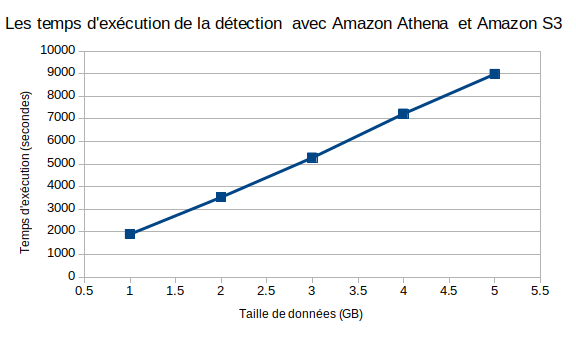
\includegraphics[width=0.7\linewidth]{illustrations/temps-avec-aws_1}
	\caption{Les temps d'exécution de la détection des anomalies en fonction de la taille de données (Amazon S3 et Amazon Athena)}
	\label{fig:temps-avec-aws}
\end{figure}


\section{Application 4 : Spark Apache avec Scala}
Nous avons implémenté l'outil de détection avec le framework Spark et l'API Scala. Les détails de l'implémentation sont donnés dans le chapitre \ref{application:spark}.  Nous avons évalué le temps d'exécution de l'outil de détection en analysant différents échantillons de traceroutes  en mode local et en mode cluster. Pour le mode local, nous avons lancer l'application Spark sur la machine ayant les caractéristiques  reprises dans la section \ref{machine-openvz-caracteritics}. Pour le mode cluster, nous avons utilisé le cluster EMR.


\subsection{Mode local}

A la base Spark est conçu pour être utilisé dans un cluster de machines sur  lequel l'analyse de données est distribuée. Toutefois, Spark peut être utilisé en mode local. Dans ce mode, on trouve le \textit{driver} et un seul \textit{executor}. Ce dernier est "lié" au même processus initié par le \textit{driver}. 


%\paragraph{Performances d'Apache Spark dans l'analyse des délais }~
Nous avons évalué le temps d'exécution de l'implémentation de l'outil de détection en utilisant Spark en variant le nombre de traceroutes à analyser. Nous avons aussi varié certains paramètres relatifs à la soumission de l'application au Spark. Nous avons varié la taille de la mémoire allouée au driver afin de choisir celle la plus adaptée. Ensuite nous avons mesuré le temps d'exécution dans le cas de local, local[K] et local[*].

\paragraph{Variant la mémoire allouée au driver}~

Dans une application Spark, la taille de la mémoire allouée pour le \textit{driver} et les \textit{executors} est  définie par défaut. D'après la documentation officielle de Spark\footnote{Source : \url{https://spark.apache.org/docs/latest/configuration.html}, consultée le $29/12/2018$.}, Spark réserve $ 1 $ GB pour le $ driver $ et $ 1 $ GB pour chaque \textit{executor}. 

En mode local (--master local), le \textit{driver} et le \textit{worker} sont liés au même processus.  Nous avons mesuré le temps d'exécution de l'application Spark en varaint la taille mémoire allouée au \textit{driver} via le paramètre \textit{driver-memory}. Par défaut, la mémoire allouée au driver est de 1 Go. Avec cette valeur, il n'est pas possible  d'analyser un ensemble de traceroutes qui fait $ 1,028,343,572 $ octets. Afin de voir l'effet de la mémoire allouée au \textit{driver}, en mode d'exécution local, nous avons utilisé deux échantillons de traceroutes. La première comprend les traceroutes capturés pendant le $ 07/02/2018 $ dans le cadre de la mesure ayant l'identifiant $ 5004 $, ce qui fait $ 1,028,343,572 $ octets (\textit{data\_1go}). Pour le deuxième échantillon, il reprend les traceroutes effectués  entre le $ 07/02/2018 $ et le $ 08/02/2018 $ effectués aussi dans le cadre de la mesure ayant l'identifiant $ 5004 $, ce qui fait $ 2,055,167,238 $ (\textit{ data\_2go}) octets.

La Figure 	\ref{fig:variantdrivermemory} présente les résultats obtenus. L'axe des abscisses indique la quantité de mémoire allouée au \textit{driver} et l'axe des ordonnées représente le temps d'exécution de détection. Pour les mêmes quantités de mémoire allouée au \textit{driver}, nous mesurons le temps d'exécution une fois pour  \textit{data\_1g}  et une autre fois pour  \textit{data\_2g}.
Pour les valeurs nulles relatives au temps d'exécution, l'exécution de la l'application a échoué. La raison de l'échec revient au manque de mémoire (message d'erreur est OutOfMemoryError: Java heap space).
\begin{figure}[H]
	\centering
	\captionsetup{justification=centering}
	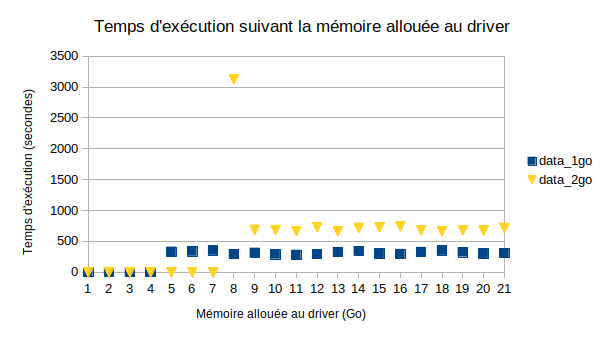
\includegraphics[width=1\linewidth]{illustrations/variant_driver_memory}
	\caption{Mesure des temps d'exécution de l'application Spark selon différentes tailles de mémoire allouées au \textit{driver} et pour deux ensembles de données différentes}
	\label{fig:variantdrivermemory}
\end{figure}

D'après la Figure 	\ref{fig:variantdrivermemory}, nous remarquons qu'à partir d'une taille mémoire allouée au driver, le temps écoulé durant l'exécution de l'application Spark est relativement stable. De plus, nous constatons qu'il faut prévoir une taille mémoire minimal pour assurer l'exécution de l'application Spark. Les tailles mémoire supérieures à cette valeur minimale affectent faiblement le temps d'exécution.  Cette valeur minimale dépend fortement de la quantité de données à analyser. Enfin, malgré que la machine sur laquelle nous lançons l'application Spark ne dispose que de $ 32 $ Go de RAM, le fait d'allouer au driver $ 35 $ Go, $ 40$ Go, $ 45 $ Go n'a pas généré une erreur lors de l'exécution.

\paragraph{Variant le mode local : local vs local[N]}~

local[*] Run Spark locally with as many worker threads as logical cores on your machine.
local [*] Exécutez Spark localement avec autant de threads de travail que de c\oe{}urs logiques sur votre ordinateur.

\paragraph{Notes concernant le mode local}~

Le mode local d'exécution d'une application Spark est typiquement utilisé pour tester le code sur une petite quantité de données dans un environnement local. Cependant, ce mode  ne fournit pas les avantages de l'environnement distribué. 

\subsection{Cluster Amazon EMR}

\paragraph{Création d'un cluster EMR}~

La création d'un cluster EMR destiné à une application Spark nécessite de  :
\begin{itemize}
	\item choisir un nom au cluster;
	\item créer la configuration du cluster;
	\item définir le modèle du n\oe{}ud maître (\textit{master}) 
	\item choisir le nombre des n\oe{}uds principaux  du cluster et leur modèle;
	\item paramétrer l'application Spark comme la précision de classe Main. 
	\item spécifier les paramètre de l'application  (.jar), l'archive se trouver dans  un compartiment Amazon S3;
	\item indiquer le chemin du compartiment Amazon S3 contenant  les données à analyser.
\end{itemize}
L'interface avancée de la création du cluster propose d'autres options.  \\

On distingue le temps nécessaire à la mise en place du cluster et la configuration du cluster (\textit{Starting}). Une fois le cluster est prêt, l'état du cluster passe à (\textit{Waiting}).  A la soumission de l'application, le cluster passe à l'état (Running). Suivant la configuration du cluster de l'utilisateur, le cluster peut s'éteindre dés la fin de l'exécution de l'application ou rester actif à l'écoute de nouvelles tâches. Toutefois, la dernière option peut produire des frais élevés.  


Avec Amazon EMR, il est possible de lancer une analyse sur le cluster et choisir l'action à appliquer à la fin de cette analyse, par exemple arrêter le cluster. Les coûts appliqués suite à l'utilisation du service Amazon EMR dépendent des caractéristiques techniques des entités du cluster, la région d'Amazon choisie du cluster et enfin le temps d'utilisation du cluster. Il est possible d'estimer les frais d'utilisation d'Amazon EMR via le calculateur disponible sur le site Web d'Amazon\footnote{Source : \url{https://calculator.s3.amazonaws.com/index.html\#s=EMR}, consultée le $14/05/2019$.}.

Nous avons utilisé l'infrastructure d'Amazon pour lancer la détection des anomalies sur un cluster de machines. Ce sont les mêmes traitements lancés dans le mode local. Nous évaluons la détection en variant deux éléments. Dans un premier temps, nous varions la taille du cluster créé pour lancer la détection. Dans ce cas, nous utilisons différents nombre d'\textit{executors}. Pour le deuxième cas, nous fixons les caractéristiques du cluster et  nous choisissons différents ensembles de traceroutes. 
Le Tableau \ref{instances-types-description} reprend les caractéristiques des instances Amazon EC2 utilisées durant nos tests. Pour chaque instance, nous avons le nombre de c\oe{}urs virtuels YARN et la taille de la mémoire.
\begin{table}[H]
	\centering
\begin{tabular}{|c|c|c|}
	\hline 
\textbf{Modèle} &	\textbf{vCores} &\textbf{	Mém. (GiB)} \\ 
	\hline 
m4.large&	$ 4 $&	$ 8 $ \\
	\hline 
m3.xlarge&	$ 8 $&	$ 15 $\\
\hline 
m4.2xlarge&	$ 16 $&	$ 32 $ \\ 
	\hline 
\end{tabular}
\caption{Description de quelques instances d'Amazon EC2}
\label{instances-types-description}
\end{table} 
\paragraph{Variant la taille du cluster}~


Le Tableau \ref{clusters-description} décrit les clusters créés au sein d'AWS EMR.  Chaque cluster reprend l'ID du cluster, le nombre d'instances formant le cluster; un \textit{driver} et  plusieurs ou aucun \textit{executor}, le type de l'instance et enfin le temps total de l'analyse. Le temps de l'analyse est calculé de la même façon  que le mode local. 



\begin{table}[H]
	\centering
	\resizebox{\textwidth}{!}{%
	\begin{tabular}{|c|c|c|c|}
	\hline 
\textbf{Nom du cluster}	&\textbf{Taille du cluster}	&  \textbf{Types d'instances (master, executor)}  &\textbf{Temps total (s)} \\ 
	\hline 
C1	&   1 &  (m4.2xlarge, --- ) &  N/A\\ 
	\hline 
C2	& 2 & (m4.2xlarge, m3.xlarge)  &240   \\ 
	\hline 
C3	& 3 &(m4.2xlarge, m3.xlarge) &225 \\ 
	\hline 
C4	& 4 & (m4.2xlarge, m3.xlarge)&217 \\ 
	\hline 
C5	& 5 & (m4.2xlarge, m3.xlarge)&134 \\ 
\hline 
C6	& 5 & (m4.large, m4.large)&  212\\ 
\hline
\end{tabular} 
}
\caption{}
\label{clusters-description}
\end{table}
De même que le mode local, on peut paramétrer le cluster avant  la soumission de l'application Spark. Etant donné que le cluster créé est destiné principalement au Spark, nous avons configuré le cluster pour utiliser toutes les ressources disponibles de mémoire, et ce à travers la propriété \textit{maximizeResourceAllocation} (voir le Listing \ref{configsparkemr}).
\begin{lstlisting}[language=json, basicstyle=\small, label= configsparkemr, caption = Exemple de fichier de configuration d'un cluster Amazon EMR]
[
{"Classification": "spark","Properties": {"maximizeResourceAllocation": "true"} },
{"Classification": "yarn-site", "Properties": {"yarn.nodemanager.vmem-check-enabled": "false"}}
]
\end{lstlisting}

\subparagraph{Description de l'ensemble de données}

%\begin{table}[H]
%	\centering
%	\begin{tabular}{|c|c|c|c|c|c|}
%		\hline 
%		Id	& Taille  & Nb. de traceroutes & Nb.liens analysé & Id. msm& période \\ 
%		\hline 
%	\end{tabular} 
%	\caption{text}
%	\label{key}
%\end{table}

%Où x4.large a les caractéristiques suivantes : (vCPU : 2, Mém. (GiB) : 8, Stockage : EBS uniquement, Bande passante dédiée à EBS (Mbit/s) : 450, Performances réseau : Modéré).

%\begin{comment}
%DelayAnalysis-one-instance : C1
%\end{comment}

%C1%https://aws-logs-847444427255-eu-west-1.s3-eu-west-1.amazonaws.com/elasticmapreduce/j-2YU5Q88TKMGBK/steps/s-H0VT3FD9TJLO/stderr.gz?
\paragraph{Variant la taille de données}~

Nous avons choisi un cluster de $ 5 $ machines afin d'évaluer plusieurs ensembles de données. Ces ensembles sont décrits dans le Tableau \ref{variantlesdonnes-fixedcluster}.
\subparagraph{Description de l'ensemble de données}~

\begin{table}[H]
	\centering
	\resizebox{\textwidth}{!}{
	\begin{tabular}{|c|c|c|c|c|c|c|}
		\hline 
		\textbf{Id}	& \textbf{Taille (Octets)}  & \textbf{Nb. de traceroutes} & \textbf{Nb.liens } &\textbf{Id. msm}& \textbf{période}&\textbf{Temps total (s)} \\ 
		\hline 
	$ S1 $	& $ 1,263,894,997 $ & $ 497,810 $ &  & $ 5008 $ & 01/05/2019 - 01/05/2019 &$ 221 $ \\ 
		\hline 
	$ S2 $	&  &  &  & $ 5008 $&01/05/2019 - 02/05/2019&  $ 415 $\\ 
		\hline 
	$ S3 $	& $ 3,792,532,958 $  & $ 1,492,196 $ &  & $ 5008 $ & 01/05/2019 - 03/05/2019 & --\\ 

\hline 
	\end{tabular} 
}
\caption{text}
\label{variantlesdonnes-fixedcluster}
\end{table}


\paragraph{Notes sur l'utilisation d'un cluster Amazon EMR}

Après avoir créé quelques clusters EMR et les évaluer sur quelques ensembles de données. Nous présentons quelques défis à soumettre. 

Le premier défi est relatif au  choix des modèles des instances. Préférer un modèle par rapport à un autre dépend des coûts, le type des traitements à appliquer sur les données et le temps qu'on admet pour avoir les résultats finaux.

La configuration du cluster est un élément clé afin d'éviter les échecs inattendus d'une analyse en cours. Cette configuration doit prendre en compte les ressources du cluster  et  la taille mémoire à allouer pour le \textit{driver}, les \textit{executors} et autres.
Enfin, le cluster créé doit évoluer avec les nouvelles données à analyser comme le cas de l'ensemble $ S3 $. C'est pourquoi la configuration de Spark doit être personnalisée pour répondre au besoin de l'application.


%https://www.knowru.com/blog/first-3-frustrations-you-will-encounter-when-migrating-spark-applications-aws-emr/
%https://dzone.com/articles/introducing-the-data-vault-alliance

\section{Récapitulatif}

Nous avons eu l'occasion d'expérimenter plusieurs technologies Big Data destinées au traitement des données massives. Ce qu'on peut apprendre d'après la pratique, c'est qu'on ne peut comparer ces technologies car elles utilisent des approches différentes et pourtant elles partagent le même objectif; analyser les données massives.

Dans la présente  discussion, nous supposons que la détection des anomalies ne se limite pas à un ensemble de données, ainsi, l'implémentation de l'outil de détection doit prendre en considération la réception de nouvelles données dans le future.



	%\item facilité de la mise en route et de la configuration de l'environnement de la technologie;
%\item flexibilité liée à la définition du  schéma de  données présentes dans les fichiers;
%\item temps d'exécution nécessaire pour fournir les résultats finaux d'une analyse de traceroutes;
%\item évolutivité de l'environnement Big Data mis en place pour des nouvelles données et de nouveaux besoins.
%mongodb

%athena
%La mise en place d'une application basée sur le service Amazon Athena nécessite le stockage de données  

%apache spark


\section{Conclusion}